\chapter{Présentation de la société}
\label{chap:introduction}
%\pagenumbering{arabic}
\section{Introduction}
\begin{figure}[h]
	
\includegraphics[scale=0.14]{./Template LaTeX/Images/cado_logo.png}
	\centering
	\caption{CADOROM}
\end{figure}
CADORIM est une société de transfert d’argent mauritanienne basée à Nouakchott,
fondée fin 2018 par un entrepreneur mauritanien, titulaire d'un doctorat en
mathématiques,
CADORIM consiste a transférer de l’argent depuis n’importe quel pays dans le
monde vers ses proches en Mauritanie. Notre objectif et de fourni une plateforme
numérique permet à l’utilisateur de régler ses commandes en toute sécurité et
confidentialité assurée par le service de PayPal qui est mondialement connu pour sa
fiabilité et simplicité.t Pour effectuer un paiement il suffit d'une simple carte bancaire
ou un compte PayPal . et une éventuelle possibilité de virement bancaire.
CADORIM a été élu comme le champion de Banque Centrale de Mauritanie (BCM )
1ère édition 2019 Fintech Challenge,
Le siège social de CADORIM est situé à marche capital , Nouakchott, Mauritanie,
immatriculée au registre du commerce.
\section{Missions}
CADORIM offre une large palette de prestations organisées autour des activités suivantes :
\begin{enumerate}
	
	\item Maintenance et amélioration de leurs propres applications (CadoRim et MauriPay)
	\item Développement des applications 
	\item Des agences des reçoivent d'argent et de service client
	
\end{enumerate}
\section{Planification du projet}
J'effectuais le diagramme de Gantt, pour avoir une meilleure compréhension de la chronologie des étapes de mon projet.
\newline
\newline
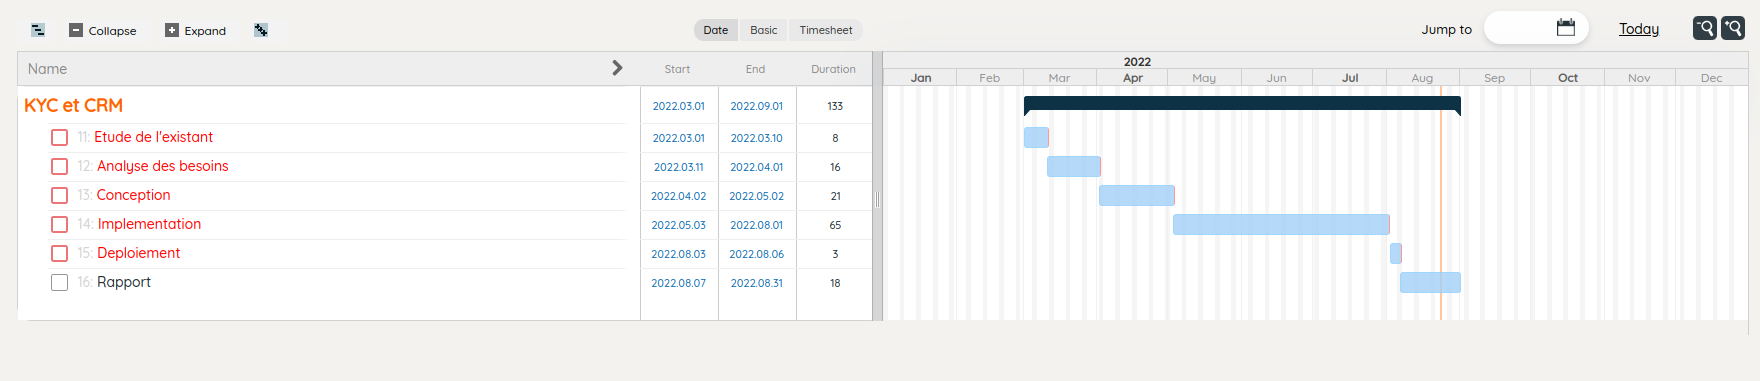
\includegraphics[width=500px,height=175px]{./Template LaTeX/Images/gantt.png}
\newline
Le projet est subdivisé en plusieurs phases.
\begin{enumerate}
\item Une phase comprenant l’étude de l’existant et analyse des besoins, en
intervenant les différents acteurs du projet.
\item Une phase de conception consistant à modéliser et formaliser les
données brutes du cahier de charge
\item Une phase d’implémentation consiste à traduire techniquement les
données provenant de la conception.
\item Déploiement : externalisation des ressources.
\end{enumerate}


